\chapter{Methodology}
\label{ch:methodology}

This chapter will address the core contributions of our project.
We present the hardware involved in \gls{sensorfusion}, describe the data acquisition procedure, then introduce our final solution, by detailing the research and implementation process, as well as design decisions that had to be made along the way.

\section{Hardware}

In this context, hardware refers to the set of sensors used for data collection, determined by the existing industrial setup. The data capturing system is controlled by an Nvidia Jetson board, which operates as a middle-man for time synchronisation between the sensors, and coordinates the various data streams. Even though the solution was designed such that it does not inherently rely on any particular device, the relationship between hardware capabilities, data quality and final output makes it crucial to understand the sensors involved in the process. Beyond the components described below, the setup includes three industrial grade ArkCam Basic+ wide angle cameras which provide a 1920x1080 RGB stream over Ethernet. These are not utilised within this project, but represent a noticeable motivation for future work directions.

\begin{figure}
	\centering
	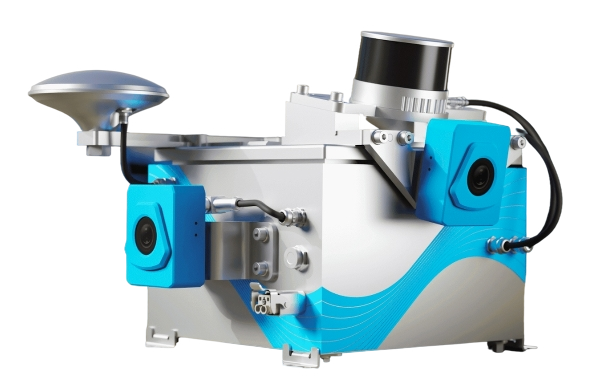
\includegraphics[width=0.6\linewidth]{images/sdx-compact-on-top-nobg.png}
	\caption[SDX-Compact]{The SDX-Compact manufactured by Sodex Innovations GmbH. The set of sensors consists of a 3D LiDAR scanner, three RGB cameras and a high-accuracy positioning system. Image source: \href{https://www.geo-lanes.com/sodex-innovations/}{GeoLanes}}
	\label{fig:sdx-compact}
\end{figure}

\subsection{LiDAR Sensor}

The SDX-Compact \reffig{sdx-compact} is equipped with a Pandar XT32 \cite{hesai_xt16_32_32m} LiDAR sensor, manufactured by Hesai Technology. This is a mechanical rotating LiDAR with a full $360 \degree$ horizontal field of view and 32 beams distributed vertically, at $1 \degree$ resolution. With our settings, the sensor produces 10 complete scans per second, resulting in a horizontal resolution of $0.18 \degree$. The maximum operational range is 120m, decreasing to 50m for low-reflectivity targets. The official specifications state a typical accuracy of $\pm 1$cm, with precision $\pm 0.5$cm, in a static environment. For each beam, the strongest return is processed, leading to 640,000 points being generated per second. The high output bandwidth is handled by an Ethernet connection, over which points are sent as \acrshort{udp} packets. The sensor also supports \acrshort{ptp} synchronisation, essential for high-quality sensor fusion.

The same device has been used for LiDAR odometry applications in the past \cite{kicp}, and has similar specifications to other popular scanners, such as Velodyne VLP-32C, Ouster OS1-32 or Robosense Helios 32.

\subsection{GNSS/INS receiver}

Another component of the sensor stack is the Septentrio AsteRx SBi3 Pro+ GNSS/INS receiver \cite{Septentrio_AsteRx_SBi3_Pro+}, which provides global positioning and orientation data at a rate of 100Hz. Internally, this relies on two distinct mechanisms.

The localization information comes from a dual antenna GNSS module compatible with several GNSS consellations (\eg \acrshort{gps}, \acrshort{glonass}, Galileo), to ensure optimal worldwide coverage. In standalone mode, the advertised typical accuracy is 1m, but the receiver also acts as an NTRIP (a protocol for differential GPS) client, gathering correction information, in order to achieve centimeter-level accuracy.

An \acrfull{imu} module records acceleration data and provides the remaining orientation angles (roll, pitch, yaw) to compute the complete pose, in 6 \acrfull{dof}. This is integrated with the absolute GNSS measurements using the patented FUSE+ technology \cite{Septentrio_FUSE_Sensor_Fusion}, resulting in an orientation error below  $\text{5-10}\degree$.

Like any system reliant on satellite communication, this will suffer significantly in situations where the signal propagation is disturbed (heavy clouds, ``urban canyons'', thick vegetation, spoofing), even leading to loss of \emph{\gls{gnssfix}}.

To conclude this section, we recognize and underline the importance of accurate extrinsic calibration between the LiDAR and the local INS coordinate frame, which has to be performed prior to any reliable data collection procedure. Given the radically different modalities of these two sensors, this is not a trivial task \cite{lidar-gps-calib} and lies outside the scope of the current work.

\begin{figure}
	\centering
	\subcaptionbox{The trajectory, overlaid on a satellite image of the region.}{
		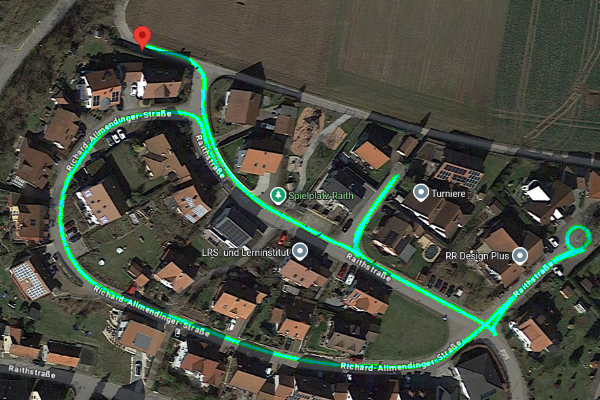
\includegraphics[width=0.45\linewidth]{images/example-trajectory.png}}
	\hspace{1pt}
	\subcaptionbox{Standard deviation of GNSS readings along the trajectory.}{
		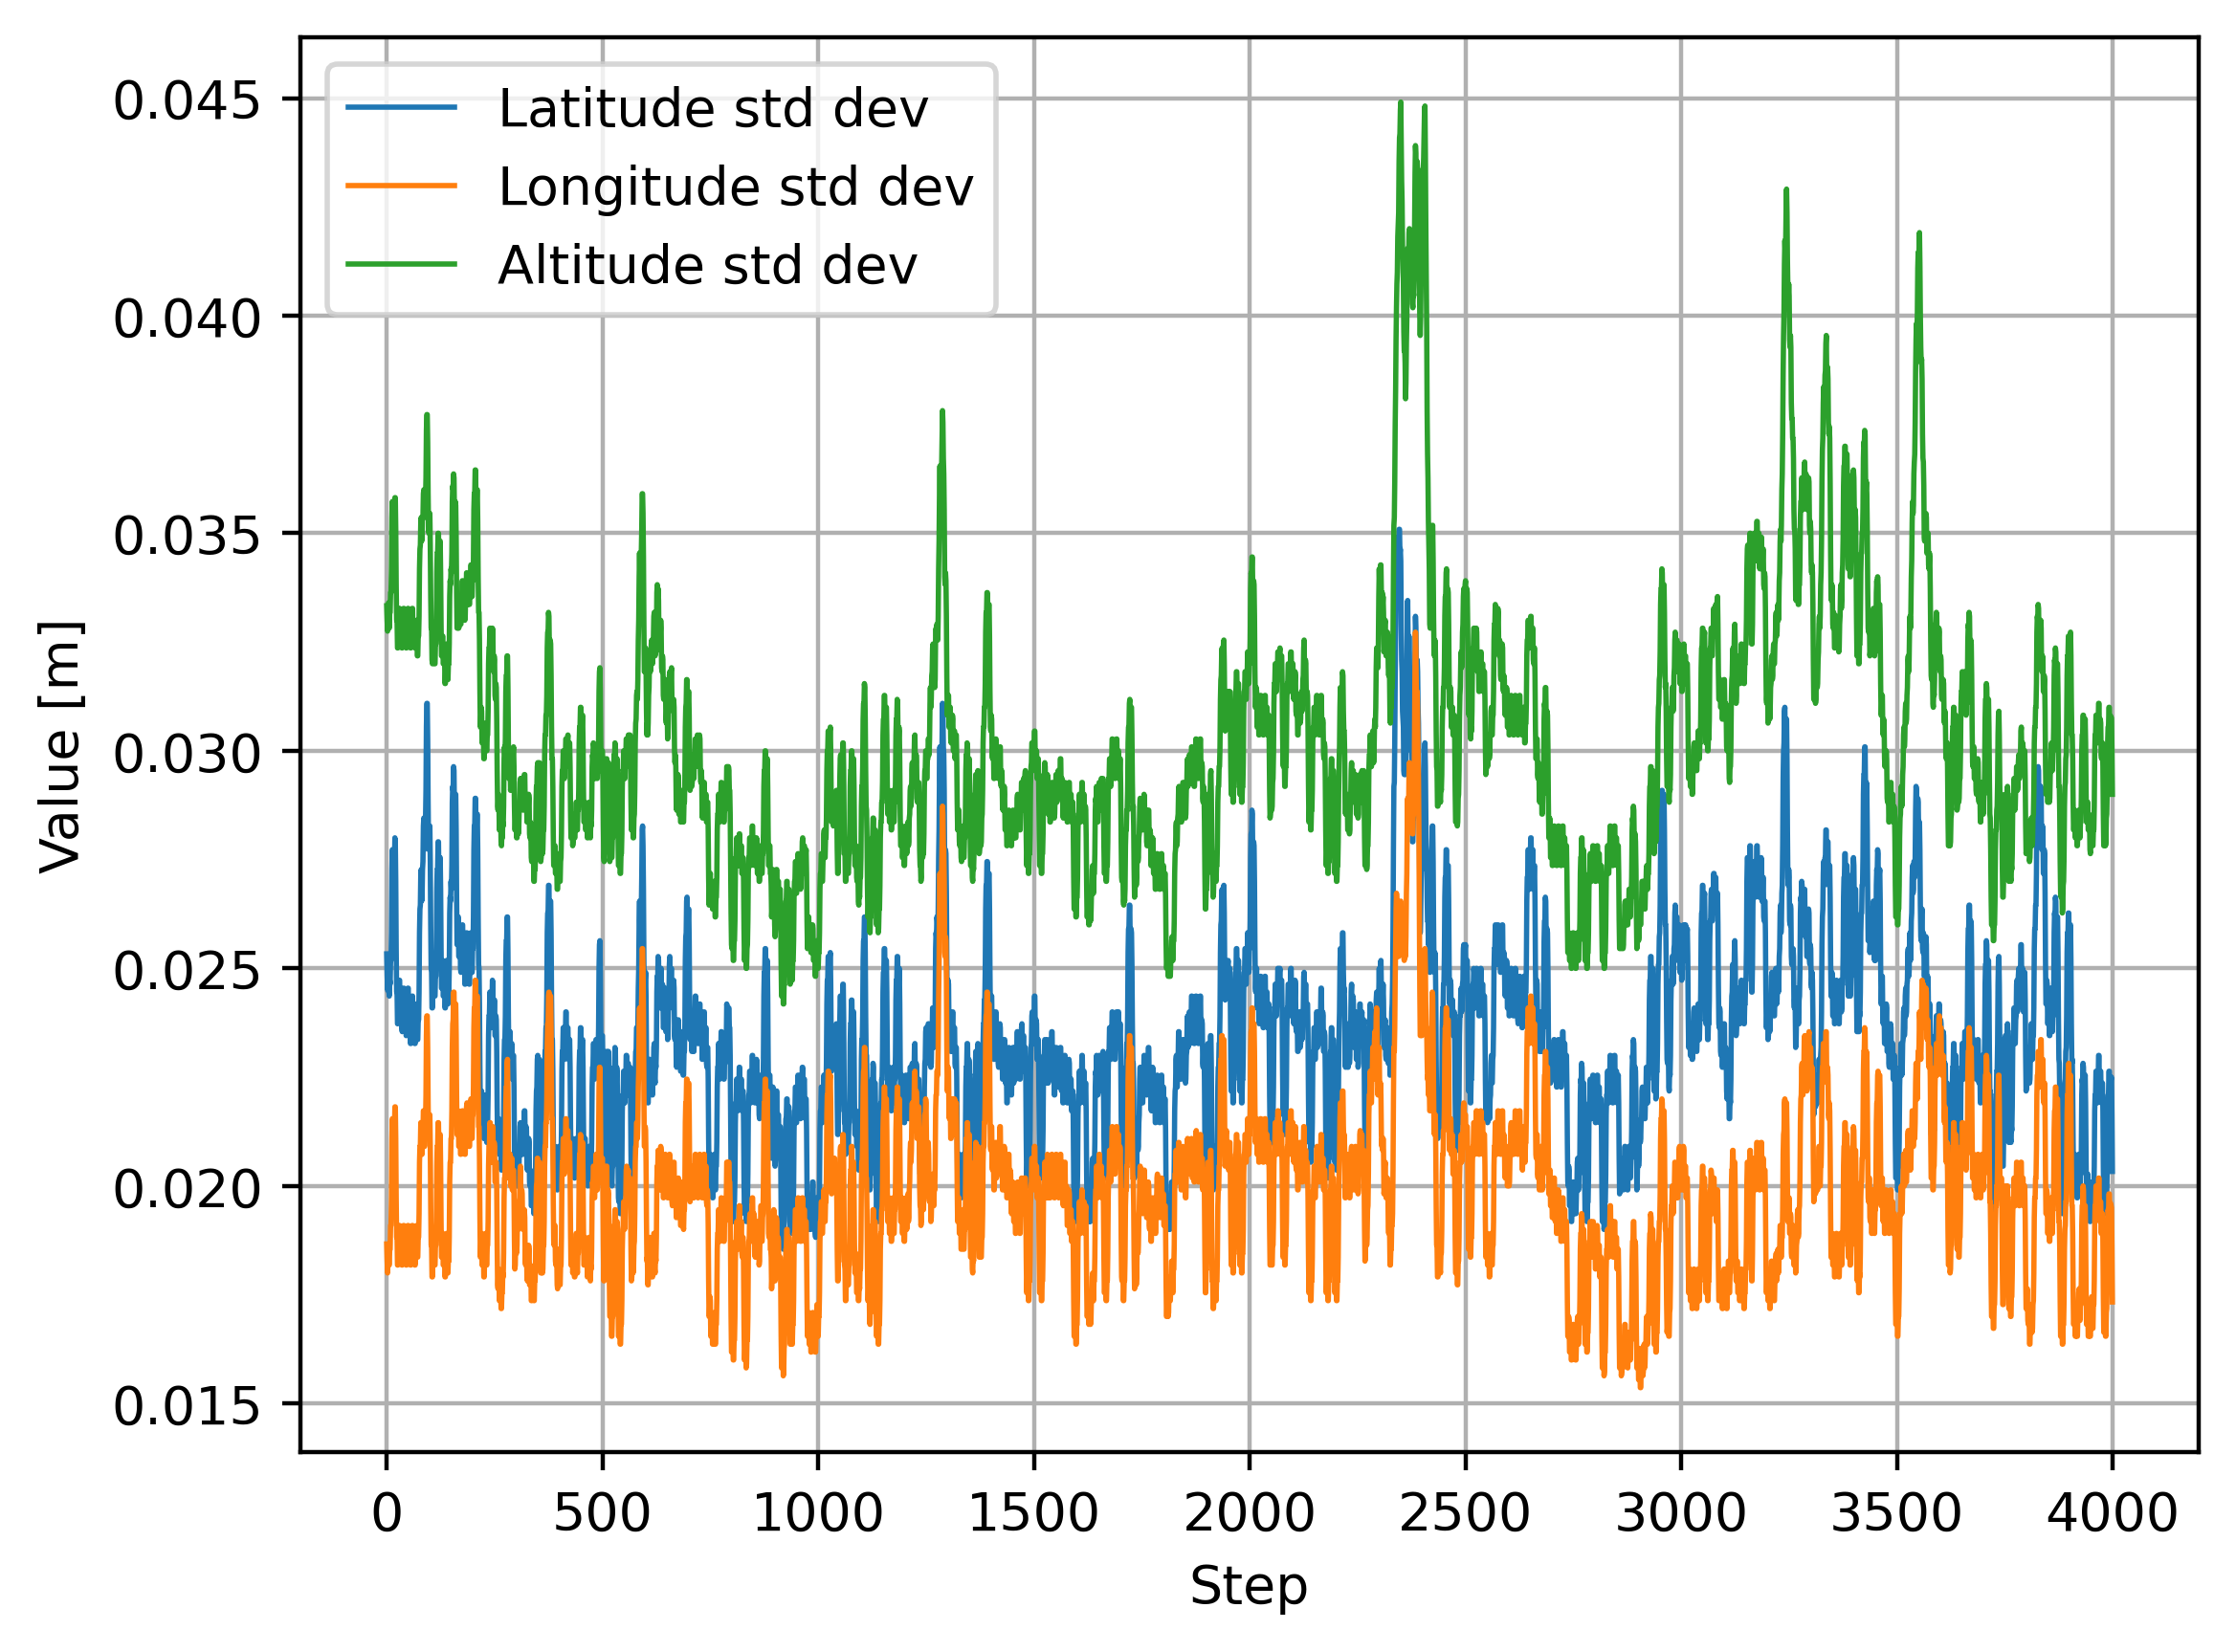
\includegraphics[width=0.45\linewidth]{images/example-trajectory-sigma.png}}
	\caption[Example dataset trajectory]{An example dataset collected in rural Germany (Lienziegen).}
	\label{fig:example-trajectory}
\end{figure}

% 48.97905882 lat
% 8.86602707 lon

\section{Data acquisition and pre-processing}

Data is collected by mounting the sensor rig on the roof of a vehicle, and driving around a target area at a relatively low speed (\eg up to 40km/h). \reffig{example-trajectory} In comparison with other public datasets \cite{nuscenes} \cite{pixset}, capturing data in non-urban environments introduces some challenges --- scenes dominated by vegetation, with few identifiable features, uneven terrain --- while minimizing others --- negligible amount of dynamic objects, no tall buildings that could affect GNSS signal propagation.

The raw sensor output is uploaded to a cloud storage facility, and is later processed into \emph{data frames} that fuse the available information \reffig{data-sync}. This can occur because the sensors are PTP-synchronized on initialization, and all recorded data is timestamped.


\begin{figure}
	\centering
	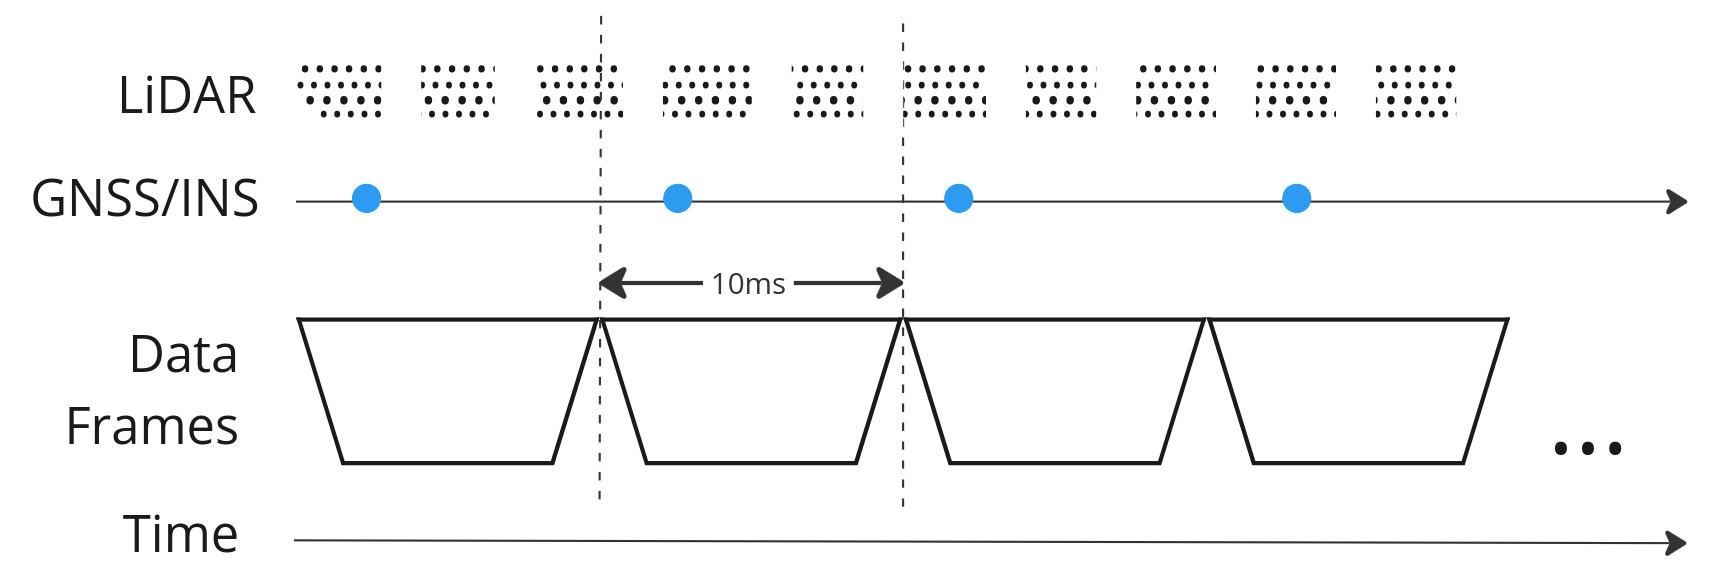
\includegraphics[width=0.7\linewidth]{images/data_sync.jpg}
	\caption[Data frame synchronisation]{The data synchronisation process.\\Time is discretized into fixed-size intervals, resulting in data frames of custom resolution. These are populated with information from the two sensors: LiDAR points arrive in groups, as UDP packets, while GNSS readings have a frequency of approx. 100Hz. We employ a data frame size of 10ms to ensure that each interval has an associated GNSS measurement, and place all corresponding packets in the same data frame.}
	\label{fig:data-sync}
\end{figure}

The next pre-processing step consists of dividing the sequence of data frames such that we operate on individual scans (also known as sweeps) produced by the LiDAR. A scan corresponds to a complete $360 \degree$ rotation, which takes 100ms, so we join the points in 10 consecutive data frames to obtain a single scan.

Every INS reading undergoes a map projection, to obtain $x,y,z$ coordinates in the East-North-Up frame. We consider the frame of the GNSS receiver as the $ego$ coordinate system. The roll $\phi$, pitch $\theta$ and yaw angles $\psi$ determine the absolute orientation, so we compute a global pose $\egoposet{} \in \SE{3}$ as:

\begin{equation}
	\notag
	\egoposet{} = \begin{bmatrix}
		\matx{R} & \vecx{t} \\ \vecx{0} & 1
	\end{bmatrix} =
	\text{Translation}(x, y, z) \cdot
	\rotmtx{z}{\psi} \cdot
	\rotmtx{x}{\theta} \cdot
	\rotmtx{y}{\phi}
\end{equation}

where $\text{Rot}_k(\alpha)$ is the transformation matrix corresponding to a rotation of $\alpha$ around axis $k$.
Because the sensor provides error estimates in the form of global one-sigma values $\left\{ \sigma_x, \sigma_y, \sigma_z, \sigma_\phi, \sigma_\theta, \sigma_\psi\right\}$, we construct the covariance matrix

\begin{equation}
	\notag
	\matx{\Sigma} = \text{diag}\left(\varx{x}, \varx{y}, \varx{z}, \varx{\phi}, \varx{\theta}, \varx{\psi}\right)
\end{equation}

and transform it using the adjoint map of the rotation component

\begin{equation}
	\notag
	\matx{\Sigma}_{ego} =
	\adjoint{\matx{R}}{\vecx{0}} \cdot
	\matx{\Sigma} \cdot
	\adjoint{\matx{R}}{\vecx{0}}^T
\end{equation}

where
\begin{equation}
	\notag
	\adjoint{\matx{R}}{\vecx{t}} =
	\begin{bmatrix}
		\matx{R}                   & \vecx{0} \\
		\skewsym{\vecx{t}}\matx{R} & \matx{R}
	\end{bmatrix}
	\text{ and }
	\skewsym{\vecx{t}} =
	\begin{bmatrix}
		0    & -t_3 & t_2  \\
		t_3  & 0    & -t_1 \\
		-t_2 & t_1  & 0
	\end{bmatrix}
\end{equation}

A LiDAR range reading $r$, captured at azimuth $\alpha$ with an elevation angle of $\phi$, can be converted to a 3D location in the LiDAR frame:

\begin{equation}
	\notag
	\lidarframe{\vecx{p}}= \begin{bmatrix}
		p_x \\ p_y \\ p_z
	\end{bmatrix}=\begin{bmatrix}
		r \cos{\phi} \sin{\alpha} \\ r \cos{\phi} \cos{\alpha} \\ r \sin{\phi}
	\end{bmatrix}
\end{equation}


If $\lidartoego$ is the pose of the LiDAR in the ego frame (from extrinsic calibration), we can compute the location of a point in the ego frame:

\begin{equation}
	\notag
	\begin{bmatrix}
		{}^{ego}\vecx{p}_\lidartxt \\ 1
	\end{bmatrix}
	= \lidartoego \begin{bmatrix}
		\lidarframe{\vecx{p}} \\ 1
	\end{bmatrix}
\end{equation}


\begin{figure}
	\centering
	\subcaptionbox{Before: an artificial duplicate surface \label{fig:motion-comp-pre}}{
		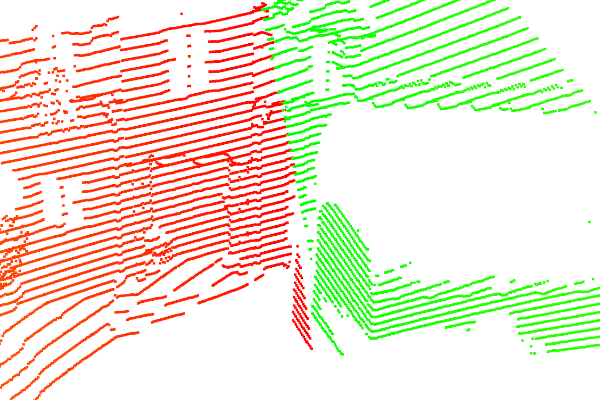
\includegraphics[width=0.45\linewidth]{images/motion-comp-pre.png}
	}
	\hspace{1pt}
	\subcaptionbox{After: surface is corrected \label{fig:motion-comp-post}}{
		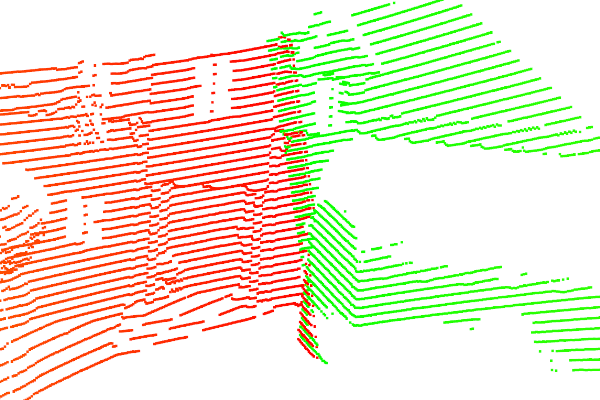
\includegraphics[width=0.45\linewidth]{images/motion-comp-post.png}
	}
	\caption[Motion compensation: before and after]{Motion artifacts and the result of motion compensation. \\Green: points from the beginning of the sweep. Red: points from the end of the sweep. Without motion compensation, the vertical surface yields two conflicting clusters, so the scan cannot be used for accurate mapping in the global frame.}
	\label{fig:motion-comp}
\end{figure}

At this stage, it is worth discussing the distortion effect that occurs when a rotating LiDAR sensor is moved at a relatively high velocity. Because it operates in a relative coordinate frame and different beams of the sweep are fired at different times, the beams corresponding to azimuth $0 \degree$ will fire approximately 100ms earlier than the beams corresponding to azimuth $359 \degree$. Placing the resulting points in the same coordinate frame would lead to undesired artifacts, such as duplicate or warped structures. \reffig{motion-comp-pre}


This open research problem \cite{motion-comp-mcdermott} is commonly addressed by estimating the sensor pose change during a sweep \cite{vicp} \cite{vizzo2023ral}, and IMU integration proves satisfactory \cite{deskewing2020}, given the short time interval involved. In our case, the ego poses
$\left\{\egoposeti{i}{0}, \egoposeti{i}{1}, \dots, \egoposeti{i}{m}\right\}$
computed from INS measurements during sweep $i$ are used to bring all points into the frame defined by $\egoposeti{i}{0}$. A point $^{i,k}\vecx{p}$ belongs to data frame $k$, so it will be replaced by:

\[
	\notag
	\begin{bmatrix}
		^{i,0}\vecx{p} \\ 1
	\end{bmatrix}
	= {}^{i,0}\pose_{i,k} \begin{bmatrix}
		{}^{i,k}\vecx{p} \\ 1
	\end{bmatrix}  = \left({\egoposeti{i}{0}}\right)^{-1} \egoposeti{i}{k} \begin{bmatrix}
		{}^{i,k}\vecx{p} \\ 1
	\end{bmatrix}
\]

We also experimented with approaches that do not rely on the absolute pose measurements for subsections of the sweep, such as interpolation using point timestamps or point indices (based on the order in which the points are returned), but these did not yield better results. A potential drawback of our method is that it disregards the localization noise, which could prove counterproductive if the GNSS receiver has low accuracy.

Through this step we are effectively removing the need for sub-scan information and creating a simpler data structure in which each scan is associated a single $\egoposet{}$ pose (from the first data frame), and the points in a sweep can be treated as a unified set.

Without loss of generality, we transform the sequence of global poses
$\left\{\posei{0}, \posei{1}, \dots, \posei{n}\right\}$
into the frame of the first pose, by multiplying each pose with  $\left(\posei{0}\right)^{-1}$, to obtain $\left\{\pose_0, \pose_1, \dots, \pose_n\right\}$. Naturally, $\pose_0$ will always be $\matx{I}_4$, which simplifies the initialization of the odometry estimation. The covariance of each pose is adjusted  with the adjoint of $\left(\posei{0}\right)^{-1}$.


% TODO write about projection

\section{Solution architecture}

At its core, the odometry and mapping solution that we propose requires minimal input: a sequence of point clouds captured by a moving LiDAR scanner, and a timestamp for each scan. If available, absolute localization/INS measurements can be used as additional input.

Let $\mathfrak{P} = \left\{ P_0, P_1, \dots P_n\right\}$ represent the set of point clouds that we operate on, with point coordinates $P_k = \left\{\vecx{p}_{k,i} \vert \vecx{p}_{k,i} \in \RR^3 \right\}$ expressed in the local frame, $\mathfrak{s} = \left\{ s_0, s_1, \dots s_n\right\}$ the corresponding timestamps, and $\widehat{\mathfrak{T}} = \left\{ \gtposei{0}, \gtposei{1}, \dots \gtposei{n} \right\}$ the ground truth poses at which each scan was captured. In an ideal setting, a point cloud registration algorithm would take $P_i$ and $P_{i+1}$ as input and return the transformation $\Delta\gtposei{i} = \gtposei{i}^{-1} \gtposei{i+1}$, \ie the ground truth displacement between consecutive poses. This would correspond to a perfect odometry model, and the complete trajectory could be reconstructed by accumulating the computed displacement. Unfortunately, with the exception of some simulation environments, such an approach is not actually feasbile. As we have already seen, LiDAR output is not perfect, especially in dynamic scenes, and some scenarios are simply unsuitable for odometry estimation based on 3D features \cite{lidartunnel}.

The output of our solution can be formulated as $\mathfrak{T} = \left\{ \pose_0, \pose_1, \dots \pose_n\right\}$. Pose $\pose_k \in \SE{3}$ represents the estimated location and orientation of the \emph{ego} frame from which the points $P_k$ were observed. The complete \emph{map} estimate, represented as a larger point cloud in global coordinates, is the set of all points, each transformed according to their respective pose:
\[
	M\left(\mathfrak{T}, \mathfrak{P}\right) =
	\left\{
	\vecx{p}_{k,i}^* \Big|
	\begin{bmatrix}
		\vecx{p}_{k,i}^* \\ 1
	\end{bmatrix} =
	\pose_k \begin{bmatrix}
		\vecx{p}_{k,i} \\ 1
	\end{bmatrix}, \vecx{p}_{k,i} \in P_k, k \in \overline{0 \dots n}
	\right\}
\]

This uncovers two possible evaluation directions, which also constitute the high-level aims of our method. On one hand, the output trajectory  $\mathfrak{T}$ should match the actual path of the system as accurately as possible. On the other, the final map $M\left(\mathfrak{T}, \mathfrak{P}\right)$ should not hide or damage small details in the scene, to obtain a high-quality 3D reconstruction. Although not immediately obvious, these can result in conflicting requirements, but they anticipate an underlying optimization problem.


\subsection{Overview}

The final architecture is the result of a series of experiments. The process began with a LiDAR-only framework, immitating the KISS-ICP \cite{vizzo2023ral} implementation. \reffig{kiss-icp-architecture} In this approach, scans are processed sequentially, attempting to compute the optimal pose at each step, and the map is built incrementally. This is computationally efficient and becomes essential when a robot operates in an unknown environment, as it provides the best localization estimates at any given time. In the absence of absolute positioning information, however, this diverges from the ground-truth trajectory \reffig{deviation-no-gps}, creating a distorted map.
\begin{figure}[h]
	\centering
	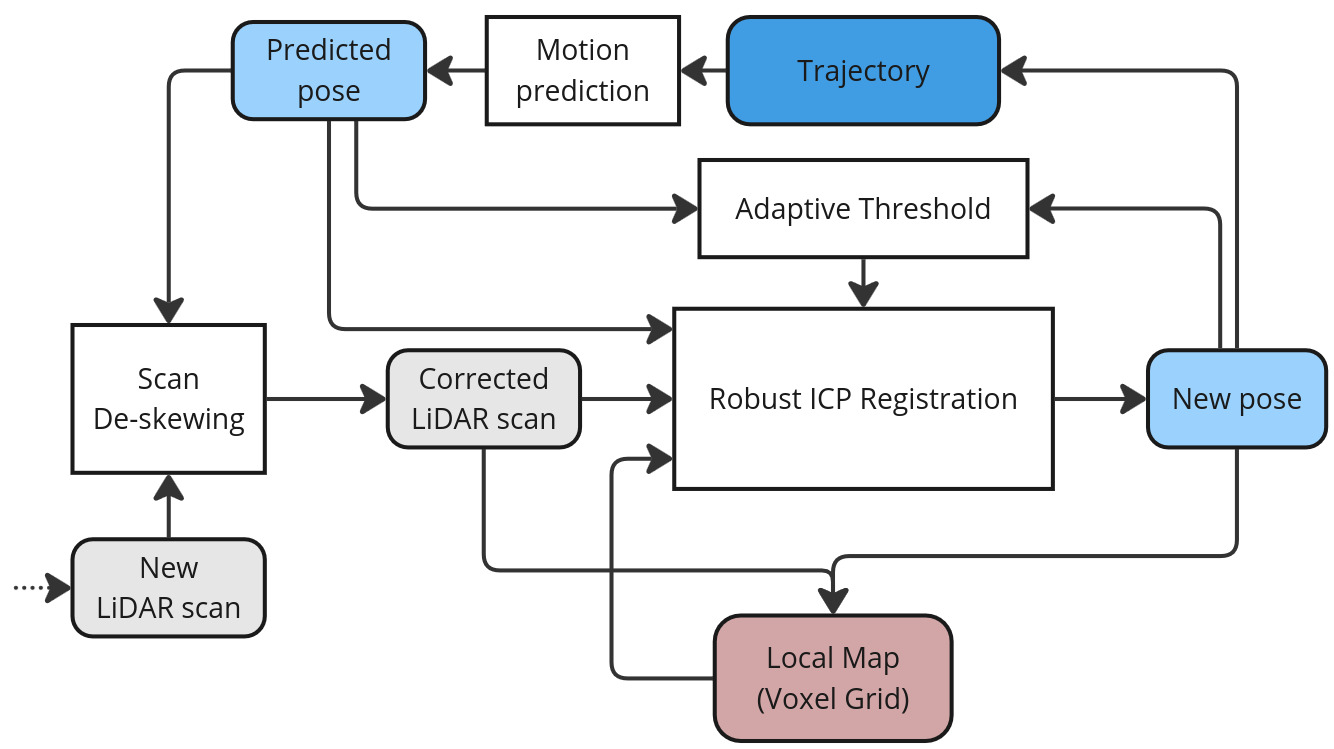
\includegraphics[width=0.6\linewidth]{images/kiss-icp-architecture.jpg}
	\caption[KISS ICP Architecture]{The KISS ICP pipeline.\\An incoming scan is motion-compensated using the displacement between the previous estimated poses, then it is downsampled and registered against the local map. The pose estimated by the ICP algorithm is added to the trajectory, and the adaptive threshold is updated by evaluating the accuracy of the motion estimation. This determines the ICP outlier removal threshold, improving the system's ability to react to unexpected motions.}
	\label{fig:kiss-icp-architecture}
\end{figure}

\begin{figure}[h]
	\centering
	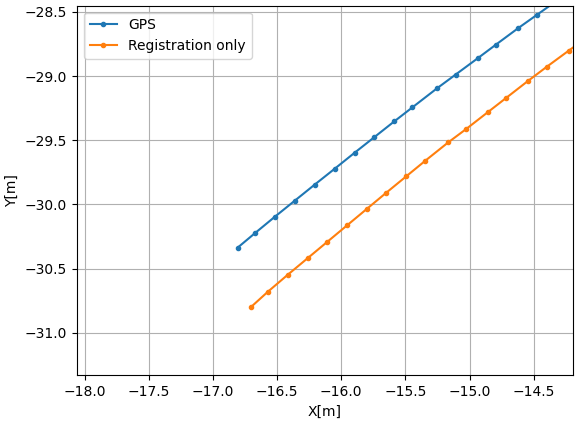
\includegraphics[width=0.45\linewidth]{images/deviation_30s.png}
	\caption[Trajectory deviation from GPS]{When the GPS information is not used, the trajectory computed based on LiDAR data diverges. Here, after 300 scans (approx. 30 seconds), the last location is approx. 0.5m away from the corresponding GPS position.}
	\label{fig:deviation-no-gps}
\end{figure}

Early efforts focused on introducing the GPS readings as a constraint at each step, alongside motion prediction and registration results. This led to experimenting with each component, as well as methods for combining the respective poses, while regularly monitoring the quality of the output trajectories and maps. As the solution was developed, it was additionally tested on more challenging scenarios, by adding artificial noise to the GPS readings, or skipping some of them altogether.

Later on, we also considered addressing the pose estimation problem holistically, instead of in an incremental fashion, and experimented with architectures based on factor graph optimization, where nodes are linked using registration and GPS constraints. The same building blocks are needed, but the relationship between them is guided by the graph paradigm. Eventually, this was adapted to obtain a hybrid solution, which combines the advantages of the two frameworks in a very intuitive manner.


\subsection{Motion prediction}

The first component that we analyse addresses the problem of predicting the next pose in the trajectory. Given the trajectory computed so far $\left\{\pose_0, \pose_1, \dots \pose_t \right\}$, we are looking for $\pose_{t+1}'$ that estimates the location and orientation of scan $P_{t+1}$ in the world frame.

This influences two other elements of the framework: motion compensation and point cloud registration. In the absence of IMU data, the displacement between consecutive scans can be interpolated to correct individual points. Point cloud registration uses this predicted pose as an initial guess, for faster convergence, as we will see in a later section.

If the scans are captured at small, equal intervals, as is usually the case for LiDAR sensors, the movement can be approximated by a constant velocity model. The displacement between the previous two scans is propagated using
$\Delta \pose_{t}' \approx \Delta \pose_{t-1} = \pose_{t-1}^{-1}\pose_{t}$, which leads to
$\pose_{t+1}' = \pose_{t} \Delta \pose_{t-1}$. In our case, the time steps are not necessarily equal, and we would like to correct this pose estimate using the GPS measurements, when available, so we experimented with a Kalman Filter for computing the location component of $\pose_{t+1}'$. The state $\bm{x}_k \sim \mathcal{N}(\kfx{k}, \kfP{k}) $ is formulated as:
\begin{align*}
	\kfx{k} & = \left[x_k, y_k, z_k, {v_x}_k, {v_y}_k, {v_z}_k\right]^T                                                    \\
	\kfP{k} & = \text{diag}\left(\varx{x_k}, \varx{y_k}, \varx{z_k}, \varx{{v_x}_k}, \varx{{v_y}_k}, \varx{{v_z}_k}\right)
\end{align*}
Over a time step $\Delta t$, this changes according to a linear model:
\newcommand{\Fdt}{\matx{F}(\Delta t)}
\newcommand{\Qdt}{\matx{Q}(\Delta t)}
\begin{align*}
	\kfxpred{k+1} & =  \Fdt \cdot \kfx{k}                    \\
	\kfPpred{k+1} & = \Fdt^T \cdot \kfP{k} \cdot \Fdt + \Qdt
\end{align*}
where
$
	\Fdt =
	\begin{bmatrix}
		\matx{I}_3 & \matx{I}_3 \Delta t \\
		\matx{0}_3 & \matx{I}_3
	\end{bmatrix}
$ and $\Qdt$ is the estimated process noise, which scales with the time interval. In the update step, we compute the new mean and covariance using a measurement $\bm{z}_k \sim \mathcal{N}(\vecx{z}_k, \matx{R})$, by applying a Kalman gain:
\begin{align*}
	\matx{K}  & = \kfPpred{k+1} \matx{H} \left(\matx{H} \kfPpred{k+1} \matx{H}^T + \matx{R}\right)^{-1} \\
	\kfx{k+1} & = \kfxpred{k+1} + \matx{K} \left(\vecx{z}_k - \matx{H}\kfxpred{k} \right)               \\
	\kfP{k+1} & = \left(\matx{I} - \matx{K} \matx{H}\right) \kfPpred{k+1}
\end{align*}

The $\vecx{z}_k$ vector consists of a location $\left[x_\text{GPS}, y_\text{GPS}, z_\text{GPS}\right]^T$ and velocity values $\frac{1}{\Delta t}\left[x_\text{GPS} - x_k, y_\text{GPS} - y_k, z_\text{GPS} - z_k\right]^T$, assuming linear displacement. The Jacobian $\matx{H}$ with respect to the state vector is $\matx{I}_6$, and the covariance of the measurement noise $\matx{R}$ can be estimated using the covariance of the GNSS reading. If no GNSS reading is associated with the current scan, the pose estimate is retrieved from the predicted position $\kfxpred{k+1}$, and the update step is performed based on the pose computed after the registration procedure.

This type of motion prediction method suffers from several disadvantages which outweigh its benefits for our use case. Firstly, it does not address the rotation component of the poses. Some possible workarounds include copying the orientation from the previous pose and letting the registration component correct that --- this has been observed to fail when a larger time gap occurs, especially for curved trajectories \reffig{reg-failure-rotation} ---, using the rotation returned by the INS, or having a separate method for computing the new rotation. Secondly, it introduces the need for reliable noise estimation \reffig{motion-model-overshoot}, such that the model is reactive to unexpected movement, while filtering out measurement noise. Process noise covariance $\matx{Q(\Delta t)}$ and the measurement input covariance $\matx{R}$ require approximations which are difficult to balance for a general solution. Therefore, using the estimated uncertainty of the predicted pose in further computations would only propagate potential sources of error.

% \begin{figure}[h]
% 	\centering
% 	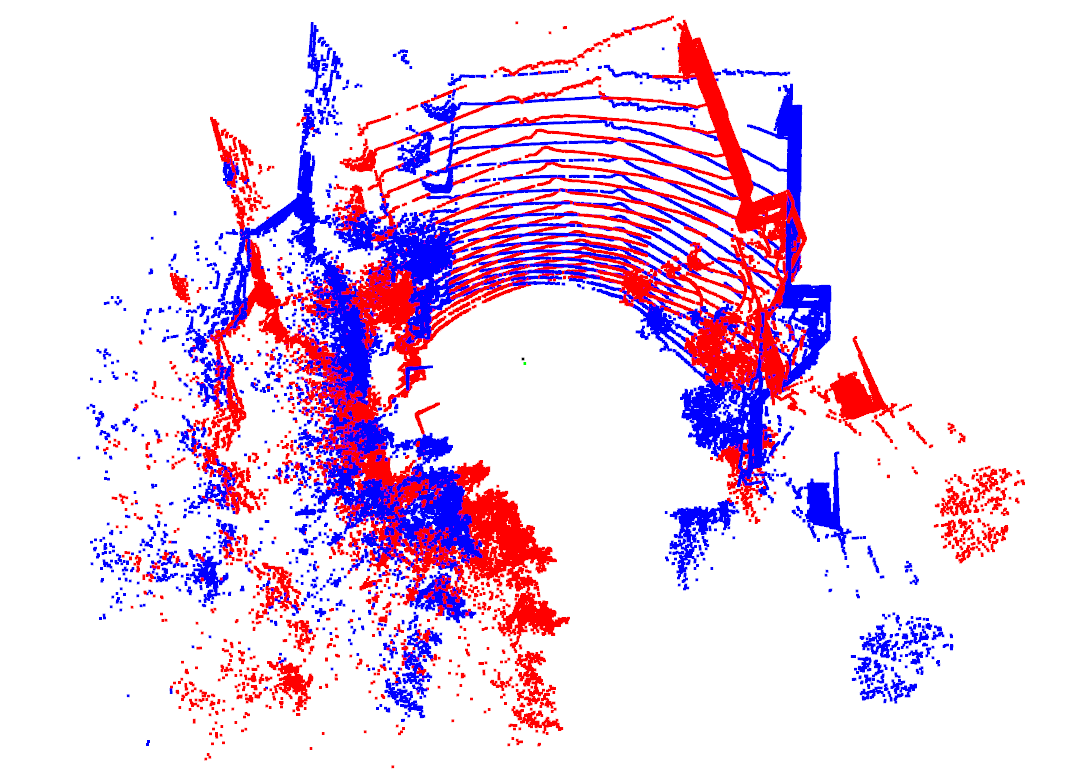
\includegraphics[width=0.5\linewidth]{images/rotation.png}
% 	\caption[Registration Failure Case (Rotation)]{Registration failure case.\\ Incorrectly estimating the rotation between scans (red and blue) can cause the registration to converge to an erroneous local minimum.}
% 	\label{fig:reg-failure-rotation}
% \end{figure}
\begin{figure}
	\centering
	\subcaptionbox{Registration failure case, when the rotation between consecutive scans (red and blue) is estimated incorrectly. \label{fig:reg-failure-rotation}}{
		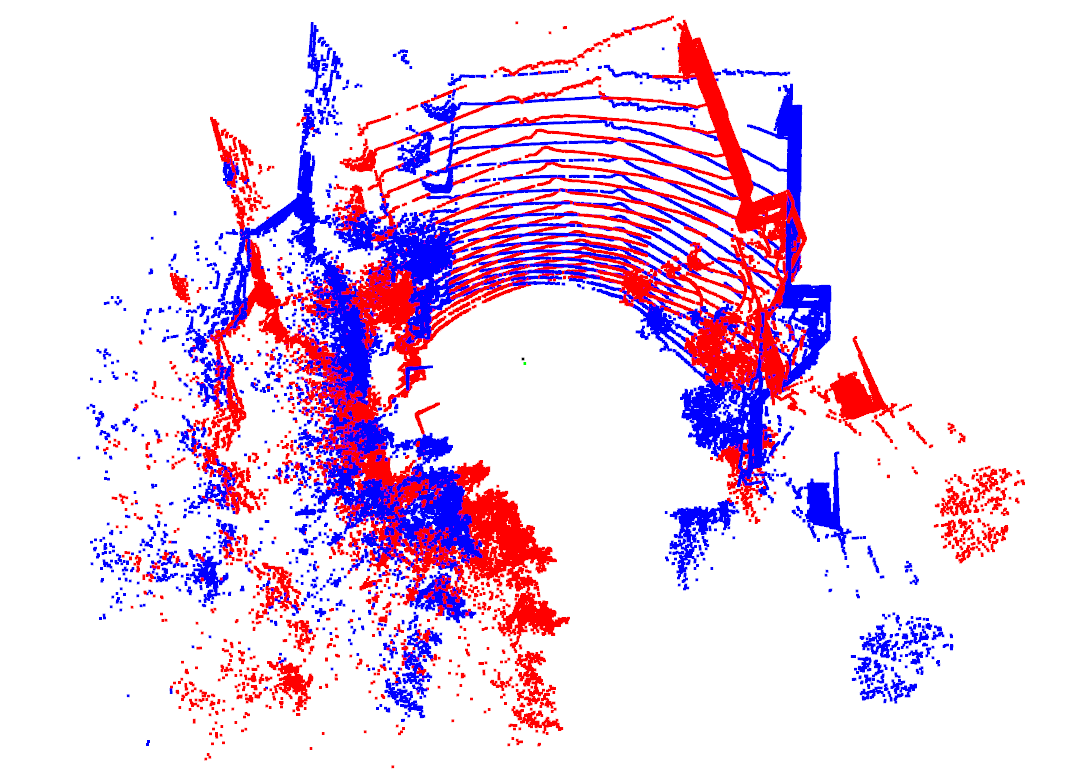
\includegraphics[width=0.47\linewidth]{images/rotation.png}
	}
	\hspace{1pt}
	\subcaptionbox{If the non-constant time intervals are ignored, the model overshoots when time gaps occur. Trajectory starts from bottom.\label{fig:motion-model-overshoot}}{
		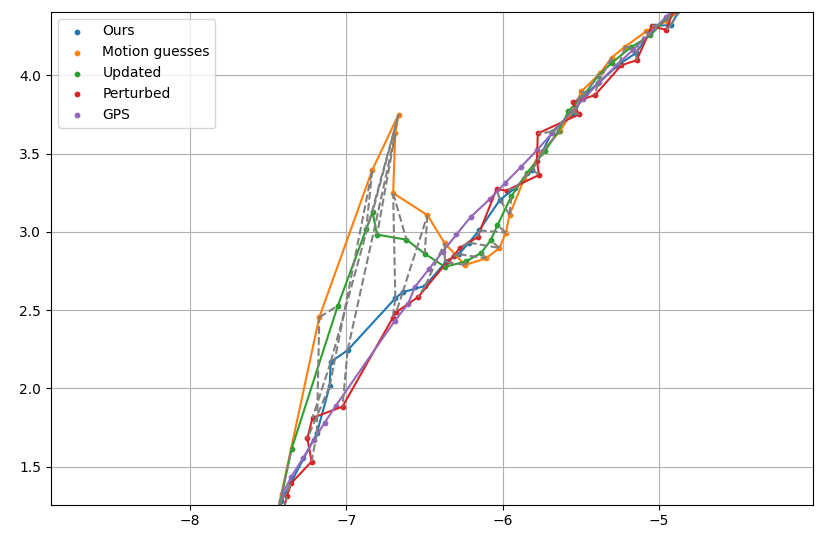
\includegraphics[width=0.47\linewidth]{images/motion-overshoot.png}
	}
	\caption[Motion model challenges]{Challenges of using a Kalman Filter motion model}
	\label{fig:motion-pred-trouble}
\end{figure}


The approach that we propose relies on the differential properties of the $\SE{3}$ manifold. For any $\matx{M} = \begin{bmatrix}
		\matx{R} & \vecx{t} \\ \vecx{0}^T & 1
	\end{bmatrix} \in \SE{3}$, there is a corresponding twist  $\widehat{\xi} = \begin{bmatrix}
		\skewsym{\vecx{w}} & \vecx{v} \\
		\vecx{0}^T         & 1
	\end{bmatrix} \in \se{3}$ which can be computed through the logarithmic map
$
	\widehat{\xi} = \logmap{\matx{M}} := \begin{bmatrix}
		\matx{V}^{-1}(\vecx{w}) \vecx{t} \\
		\LogSO{\matx{R}}
	\end{bmatrix}
$,
where
$\matx{V}(\vecx{w}) = \matx{V}(\theta\vecx{u})  := \matx{I}_3 + \frac{1-\cos\theta}{\theta}\skewsym{\vecx{u}} + \frac{\theta-\cos\theta}{\theta}\skewsym{\vecx{u}}^2$. The inverse operation, the exponential map, is defined as
$
	\matx{M} = \expmap{\widehat{\xi}} := \begin{bmatrix}
		\ExpSO{\vecx{w}} & \matx{V}(\vecx{w})\vecx{v} \\
		\matx{0}         & 1
	\end{bmatrix}
$. $\LogSO{}$ and $\ExpSO{}$ are the logarithmic and exponential maps that convert between $\vecx{w} \in \RR^3$ and $\matx{R} \in \SO{3}$. All of this allows the introduction of an interpolation function, with a parameter $t \in \left[0, 1\right]$:
\newcommand{\Mtx}[1]{\matx{M}_{#1}}
\[
	\varphi\left(\Mtx{1}, \Mtx{2}, \alpha\right) :=
	\Mtx{1} \expmap{\alpha \cdot \logmap{\Mtx{1}^{-1} \Mtx{2}}}
\]

In our case, using $\pose_{t-1}$ and $\pose_{t}$ to compute $\pose_{t+1}'$ is actually a matter of extrapolation, because we expect $\alpha$ to be approximately 2 at most steps, which would lead to unstable behaviour in the Lie group transformation. To avoid this, we first compute $\pose_{t+1}'' = \pose_{t}\pose_{t-1}^{-1}\pose_{t}$, and then obtain $\pose_{t+1}' = \varphi\left(\pose_t, \pose_{t+1}'', \alpha_{t}-1\right)$, where $\alpha_{t}= \frac{s_{t+1} - s_{t-1}}{s_t - s_{t-1}}$.


%% diagram of initial architecture

% mention gaps in the data
% sequential framework - advantages, need for pose at every step
% explain registration equations
% explain map creation
% describe motion model experiments
% describe attempts to include GPS measurements
% - interpolation with fixed alpha
% - combination weighted by covariances
% describe issues - deviation, equal time steps, unable to correct past poses, when GPS is received
% 
% 

%% fix dots in enumerations

% Similarly, $M\left(\widehat{\mathfrak{T}}, \mathfrak{P}\right)$ represents the ground truth map.



% The challenge lies in 

% \begin{compactitem}
% 	\item The trajectory described by this sequence matches the path of the system in the real world as accurately as possible
% 	\item The full point cloud,
% \end{compactitem}

% intermediate challenge = get as good of a displacement estimate, despite the noise in the data


